\documentclass[%
    10pt,
    professionalfont,
    aspectratio=169,
%    handout,
    xcolor=dvipsnames, 
]{beamer}

\mode<presentation>{%
    \usetheme[alternativetitlepage=bild]{Rub}
    \titlegraphic{img-bg-rub.jpg}
    \setbeamercovered{invisible}
}
\usepackage{pgfpages}
%\setbeameroption{show notes on second screen}
\setbeamertemplate{theorems}[numbered]

\usepackage{rubfonts2009}
%\usepackage[scaled]{berasans}
\usepackage[charter]{mathdesign}
\SetMathAlphabet{\mathcal}{normal}{OMS}{zplm}{m}{n}

\usepackage[utf8]{inputenc}
\usepackage[T1]{fontenc}

\usepackage{fontawesome}

\usepackage{graphicx}
\definecolor{gelbgruen}{cmyk}{0.5,0,1,0}
\definecolor{lichtgrau}{cmyk}{0.03,0.03,0.03,0.1}
\definecolor{saphierblau}{cmyk}{1,0.5,0,.6}
\definecolor{ucorange}{cmyk}{0,0.45,0.93,0.04}
\definecolor{alertred}{rgb}{0.80,0.12,0.12}

\usepackage{abbrv}
\usepackage{delimiters}

\usepackage[english]{babel}
\usepackage{csquotes}

\usepackage{amsmath}
\usepackage{mathtools}

\usepackage{etoolbox,siunitx}
\sisetup{binary-units}

\usepackage{booktabs}

\usepackage{setspace}
\usepackage{todonotes}

\usepackage{algorithm}
\usepackage[noend]{algpseudocode}
\newcommand*\Let[2]{\State{} #1 $\gets$ #2}
\algrenewcommand\alglinenumber[1]{%
    {\sffamily\footnotesize#1}}
\algrenewcommand\algorithmicrequire{\textbf{Input:}}
\algrenewcommand\algorithmicensure{\textbf{Output:}}

\usepackage{accsupp}
\usepackage{listings}

\newcommand{\noncopynumber}[1]{%
    \BeginAccSupp{method=escape,ActualText={}}
    #1
    \EndAccSupp{}
}

\usepackage{tikz}
\usepackage{tikzsymbols}
\usetikzlibrary{backgrounds}
\usetikzlibrary{calc}
\usetikzlibrary{positioning}
\usetikzlibrary{decorations.pathreplacing, overlay-beamer-styles}
\usetikzlibrary{shapes}
\usetikzlibrary{matrix}

\usetikzlibrary{chains,shapes.arrows,fit}
\definecolor{arrowcolor}{RGB}{201,216,232}% color for the arrow filling
\definecolor{circlecolor}{RGB}{79,129,189}% color for the inner circles filling
\colorlet{textcolor}{white}% color for the text inside the circles
\colorlet{bordercolor}{white}% color for the outer border of circles

\usetikzlibrary{crypto.symbols}
\tikzset{shadows=no}        % Option: add shadows to XOR, ADD, etc.
\usepackage{pgfplots}
\usetikzlibrary{pgfplots.colormaps}


\newcommand{\repeatarrow}{%
    \begin{tikzpicture}[inner sep=0pt, baseline=(base)]%
    \node (n) {};
    \draw[thick,<-] (n.center) ++(110:0.6em) arc (110:430:0.6em);
    \node (base) at (0,-.5ex) {};
    \end{tikzpicture}%
}

\usepackage[beamer]{hf-tikz}
\usepackage{forest}

\tikzset{%
    invisible/.style={opacity=0,text opacity=0},
    visible on/.style={alt={#1{}{invisible}}},
    alt/.code args={<#1>#2#3}{%
        \alt<#1>{\pgfkeysalso{#2}}{\pgfkeysalso{#3}} % \pgfkeysalso doesn't change the path
    },
    marked/.style={
        color=alertred,
    },
    marked on/.style={alt=#1{marked}{}},
}
\forestset{%
    visible on/.style={%
        for tree={%
            /tikz/visible on={#1},
            edge+={/tikz/visible on={#1}}
        }
    }
}

\def\colorize<#1>{%
    \temporal<#1>{\color{black}}{\color{alertred}}{\color{black!50}}%
}



\pgfdeclarelayer{background}
\pgfsetlayers{background,main}

\colorlet{arrowcolor}{saphierblau}
\colorlet{circlecolor}{white}
\colorlet{bordercolor}{gelbgruen}
\colorlet{textcolor}{saphierblau}


\hypersetup{%
    colorlinks=true,
    citecolor=black!70!green,
    linkcolor=black!70!red,
    urlcolor=black!20!blue,
}

\newrobustcmd*{\fullfullcite}{%
    \AtNextCite{%
        \AtEachCitekey{%
            \defcounter{maxnames}{99}%
            \DeclareNameAlias{labelname}{given-family}%
        }%
    }%
    \fullcite
}

\newcommand{\blfootnote}[1]{%
    \begingroup
        \renewcommand\thefootnote{}\footnote{#1}%
        \addtocounter{footnote}{-1}%
    \endgroup
}
\newcommand{\vpPp}{\vphantom{Pp}}
\newcommand{\coset}[2]{#1 \!\! + \!\! #2}
\newcommand{\through}[1]{\stackrel{#1}{\rightarrow}}
\newcommand\tower[2]{\genfrac{}{}{0pt}{}{#1}{#2}}
\DeclareMathOperator*{\Prob}{Pr}

\newcommand{\F}{\mathbb{F}}
\newcommand{\derive}[2]{\Delta_{#1}\parens{#2}}
\renewcommand{\iprod}[2]{\angles{#1, #2}}
\DeclareMathOperator*{\diffOp}{\rightarrow}
\newcommand{\propDiff}[4]{#1 \diffOp^{#2}_{#3} #4}
\DeclareMathOperator{\ImOp}{Im}
\renewcommand{\Im}[1]{\ImOp {#1}}
\DeclareMathOperator{\SpanOp}{Span}
\newcommand{\Span}[1]{\SpanOp\set{#1}}

\makeatletter
\def\maxwidth#1{\ifdim\Gin@nat@width>#1 #1\else\Gin@nat@width\fi}
\def\maxheight#1{\ifdim\Gin@nat@height>#1 #1\else\Gin@nat@height\fi}
\makeatother

\def\printcipher/{PRINTcipher}
\def\robin/{Robin}
\def\iscream/{iSCREAM}
\def\scream/{SCREAM}
\def\midori/{Midori}
\def\misty/{Misty}
\def\zorro/{Zorro}
\def\spook/{\textsf{Spook}}
\def\clyde/{Clyde}
\def\shadow/{Shadow}

\title{Security Arguments and\\ Tool-based Design of Block Ciphers}
\author{Friedrich Wiemer}
%\institute{%
%    Robert Bosch GmbH, AE-BE/ECS
%}

\date[April 6th, 2020]{\small{}April 6th, 2020}

\begin{document}

\begin{frame}[plain]
    \titlepage{}
\end{frame}

\section{Introduction}
\begin{frame}{Me}
    \begin{columns}
        \begin{column}{0.3\textwidth}
            \centering
            \visible<1->{
                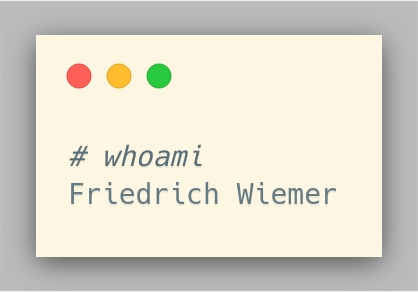
\includegraphics[width=\textwidth]{data/whoami.png}
            }
            \vspace{-10pt}
            \visible<2->{
            \begin{block}{Private}
                \Large
                \hspace{15pt} \faCameraRetro
                \hspace{17pt} \raisebox{-3pt}{
\includegraphics[width=20pt]{data/sailingboat.png}}
                \hspace{10pt} \raisebox{-3pt}{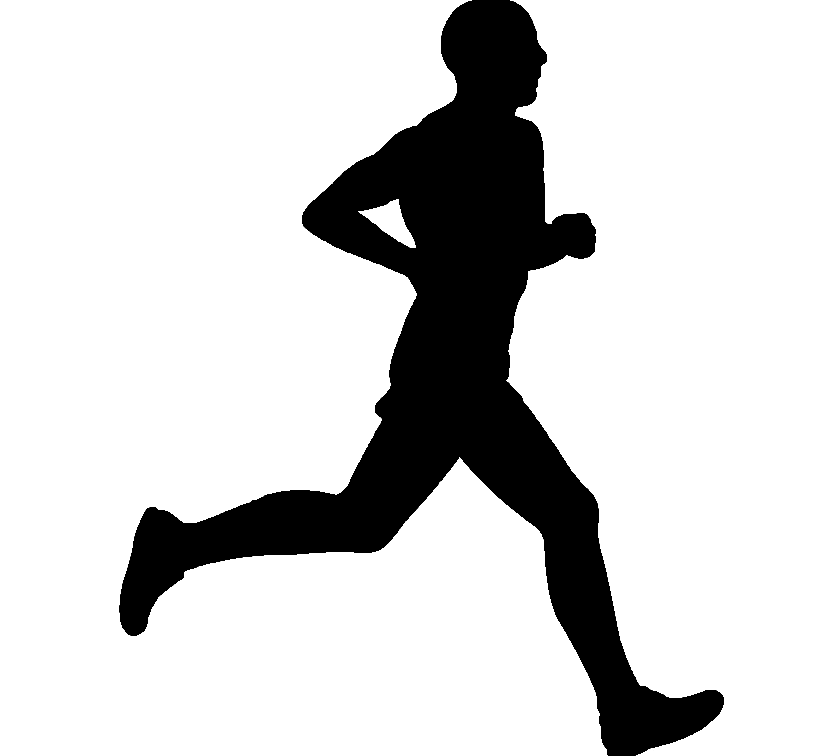
\includegraphics[width=20pt]{data/runner.png}}
            \end{block}
            }
        \end{column}
        \hspace{50pt}
        \begin{column}{0.4\textwidth}
            \visible<3->{
            \setbeamercolor{block body}{use=structure,fg=black,bg=white!20!white}
            \begin{block}{IT-Security at Ruhr Uni Bochum}
            \centering
            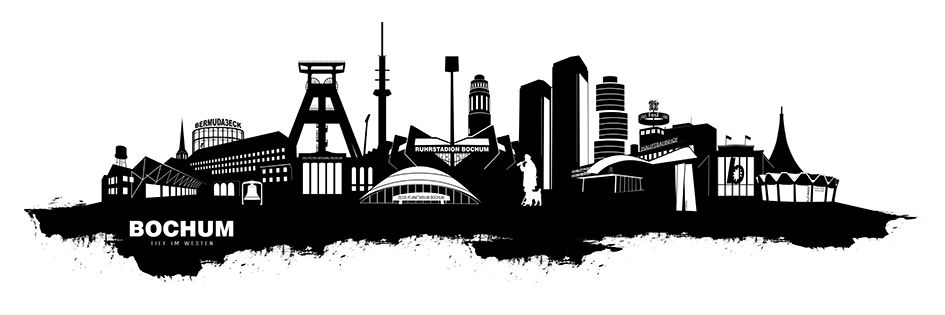
\includegraphics[width=\textwidth]{data/bochum-skyline.jpg}
            \end{block}
            }
        \end{column}
    \end{columns}
    \begin{columns}
        \begin{column}{0.475\textwidth}
            \visible<4->{
            \begin{block}{Doctoral Studies}
                Topic:\\
                Design \& Analysis of Block Ciphers \emph{for the IoT}
            \end{block}
            }
        \end{column}
        \begin{column}{0.45\textwidth}
            \visible<5->{
            \vspace*{-15pt}
            
\includegraphics[width=\textwidth]{data/cryptosolutions.png}
            }
        \end{column}
    \end{columns}
\end{frame}

\begin{frame}{\faCameraRetro}{Analogue}
    \centering
    \begin{tikzpicture}
    \matrix (m) [matrix of nodes, ampersand replacement=\&] {
        \node {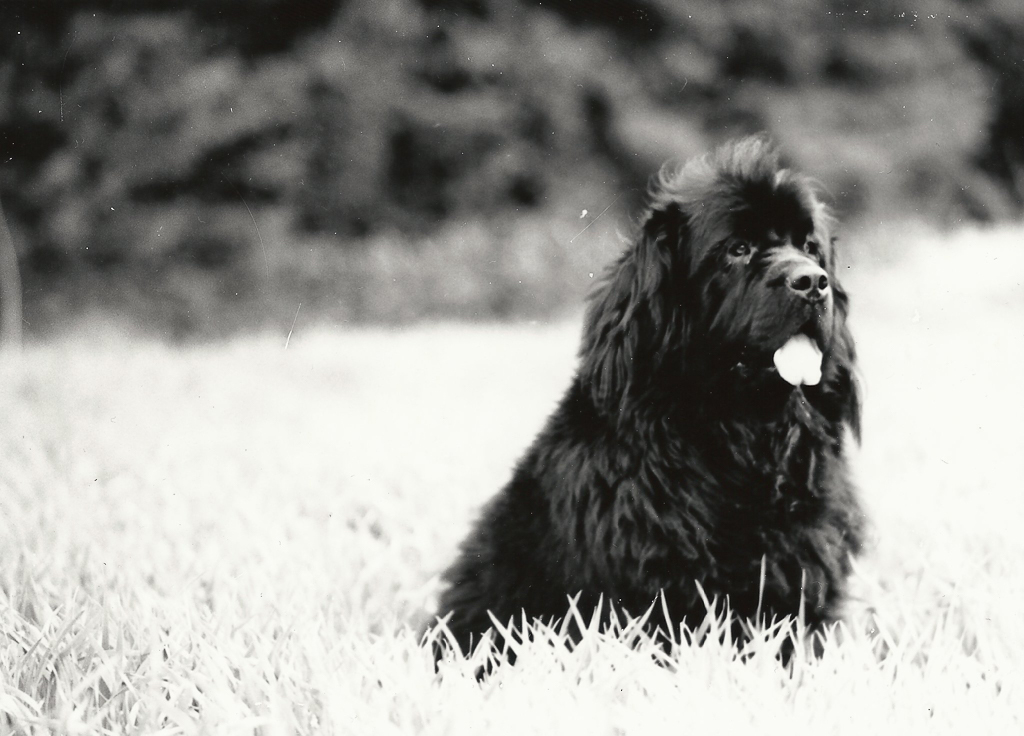
\includegraphics[height=100pt]{data/animals-0001.jpg}}; \&
        \node {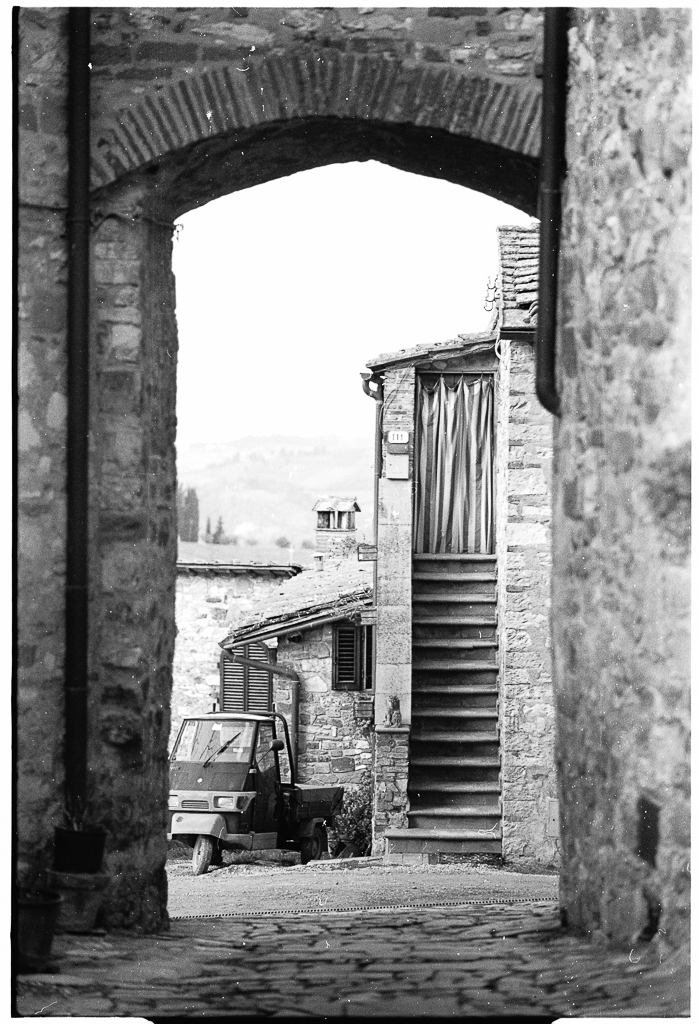
\includegraphics[height=100pt]{data/architecture-0002.jpg}}; \&
        \node {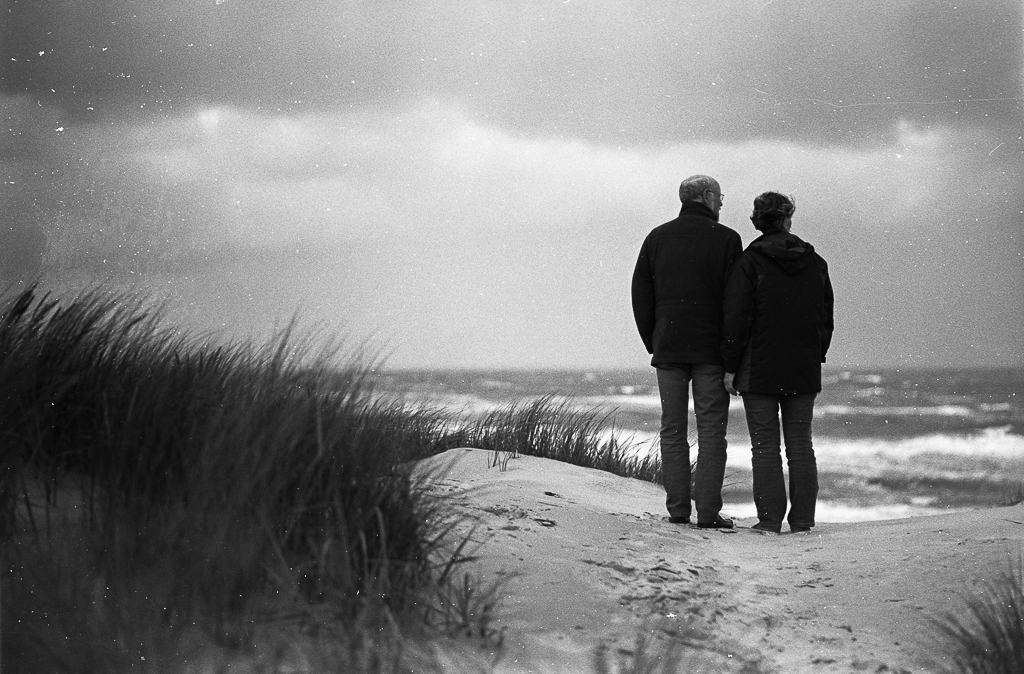
\includegraphics[height=100pt]{data/misc-0005.jpg}}; \\
    };
    \end{tikzpicture}
\end{frame}

\begin{frame}{\faCameraRetro}{Digital}
    \centering
    \begin{tikzpicture}
    \matrix (m) [matrix of nodes, ampersand replacement=\&] {
        \node {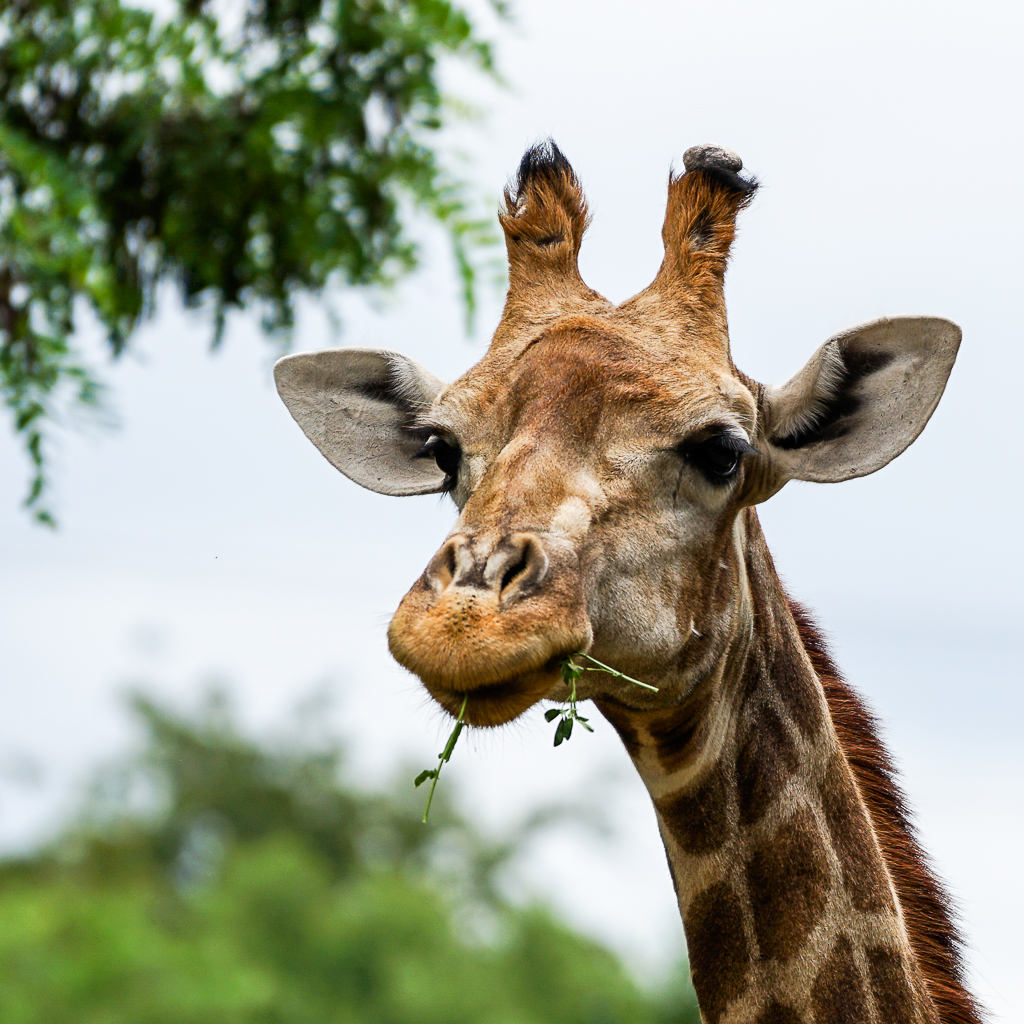
\includegraphics[height=80pt]{data/animals-0007.jpg}}; \&
        \node {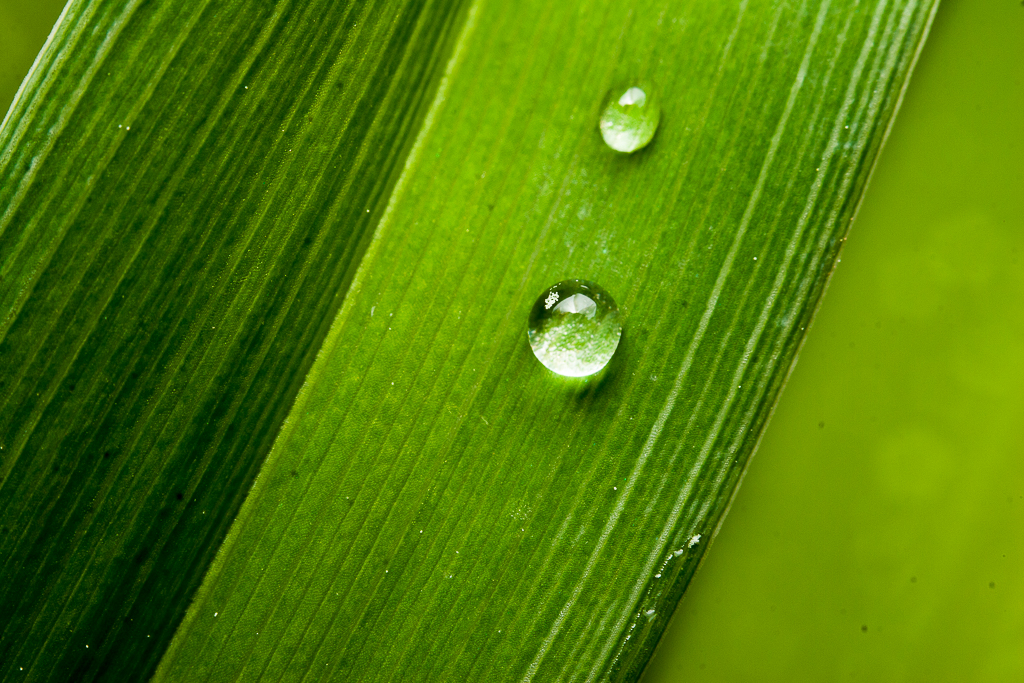
\includegraphics[height=80pt]{data/macro-0003.jpg}}; \&
        \node {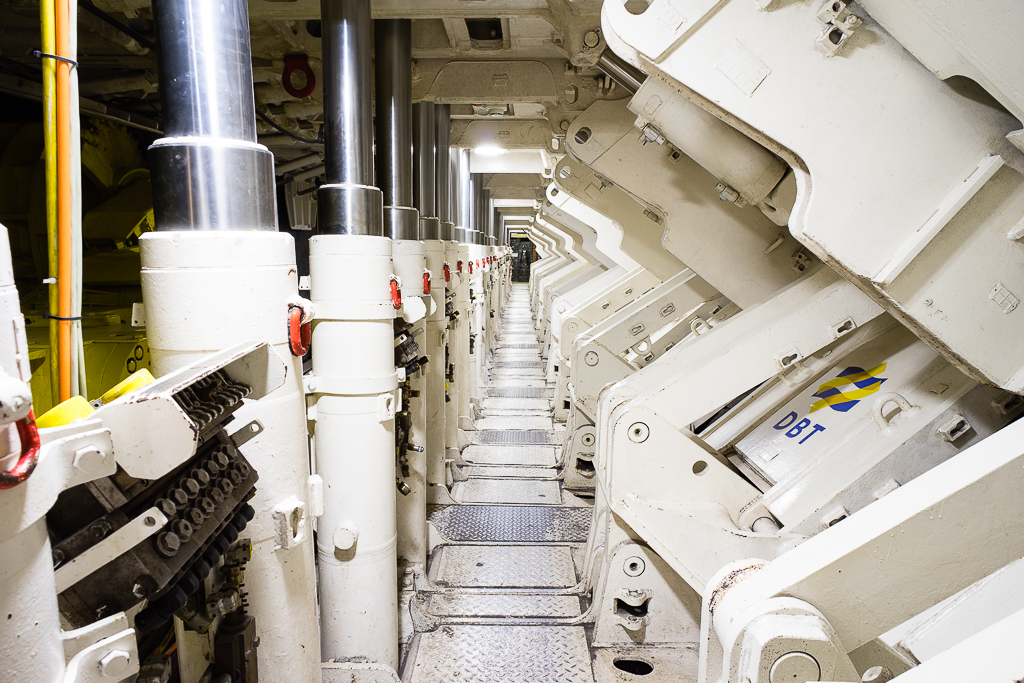
\includegraphics[height=80pt]{data/misc-0011.jpg}}; \\
        \node {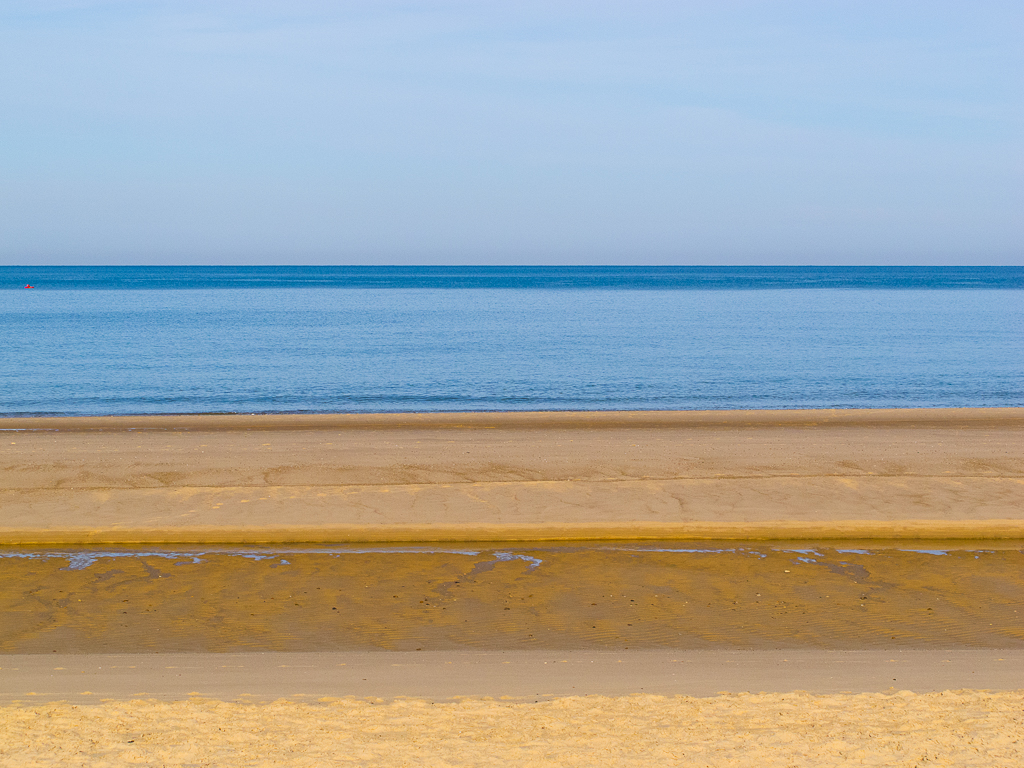
\includegraphics[height=80pt]{data/nature-0002.jpg}}; \&
        \node {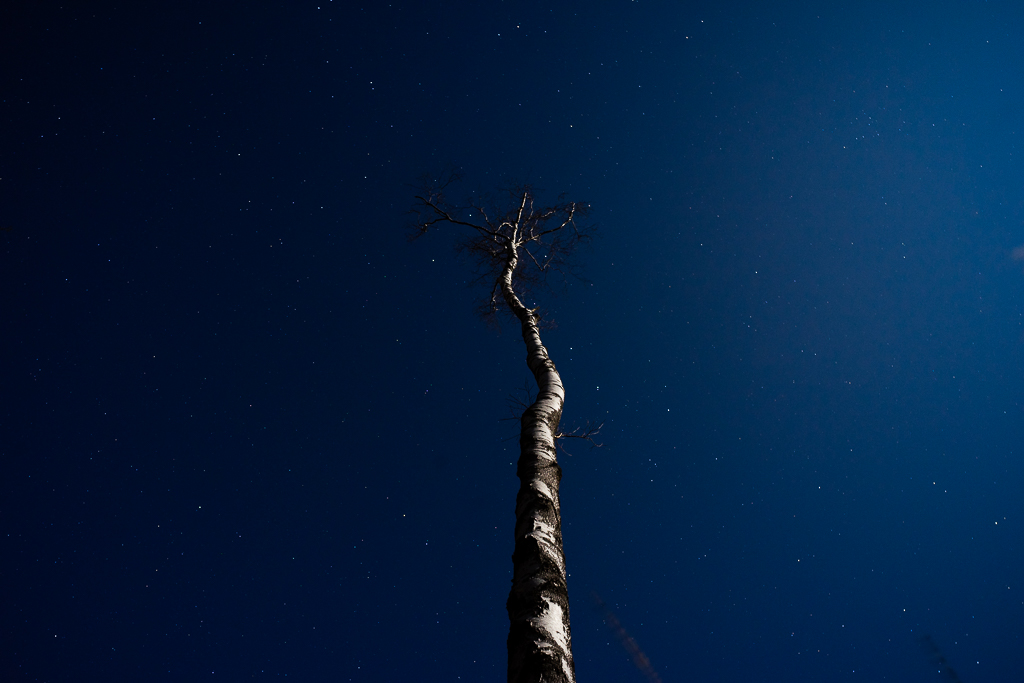
\includegraphics[height=80pt]{data/nature-0009.jpg}}; \&
        \node {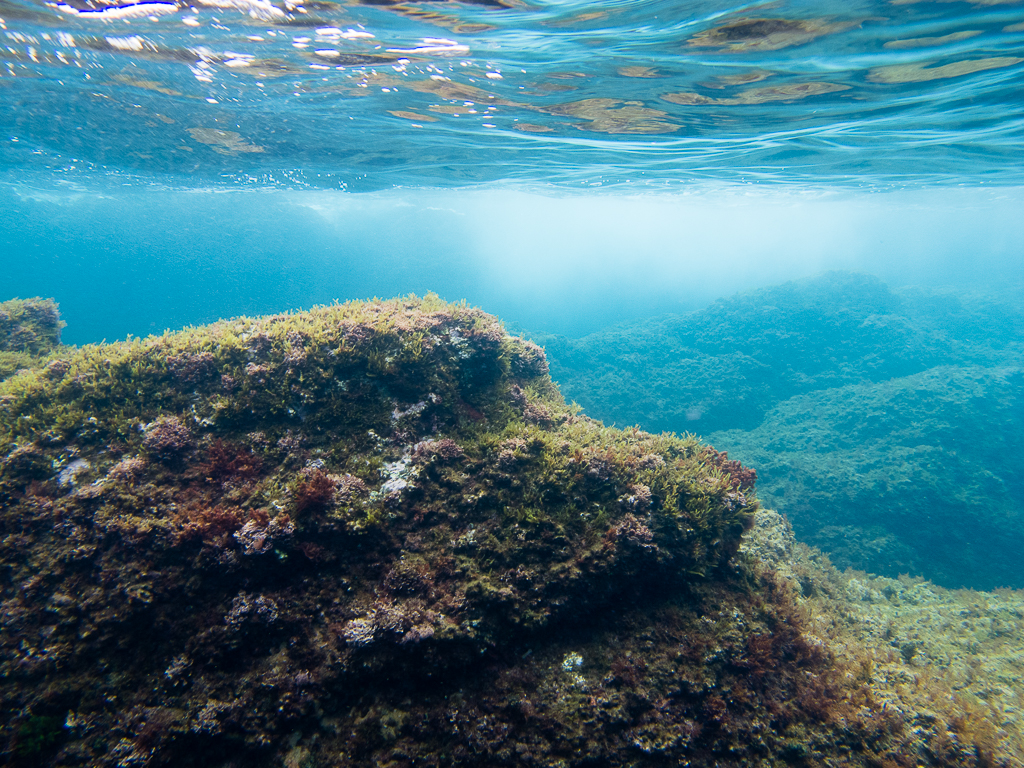
\includegraphics[height=80pt]{data/nature-0016.jpg}}; \\
    };
    \end{tikzpicture}

    {\small \href{https://asante.dev/photos}{asante.dev/photos}} \hspace{10cm}
\end{frame}

\begin{frame}{Research}
    \begin{columns}
        \begin{column}{0.45\textwidth}
            \begin{itemize}
                \item \enquote{High-Speed Implementation of bcrypt Password Search using Special-Purpose Hardware}
                \item \enquote{Parallel Implementation of BDD enumeration for LWE}
                \item \enquote{Out of Oddity -- New Cryptanalytic Techniques against Symmetric Primitives Optimized for Integrity Proof Systems}
            \end{itemize}
        \end{column}
        \begin{column}{0.45\textwidth}
            \setbeamercolor{block body}{use=structure,fg=black,bg=white!20!white}
            \begin{block}{Topics besides PhD Thesis}
            \centering
            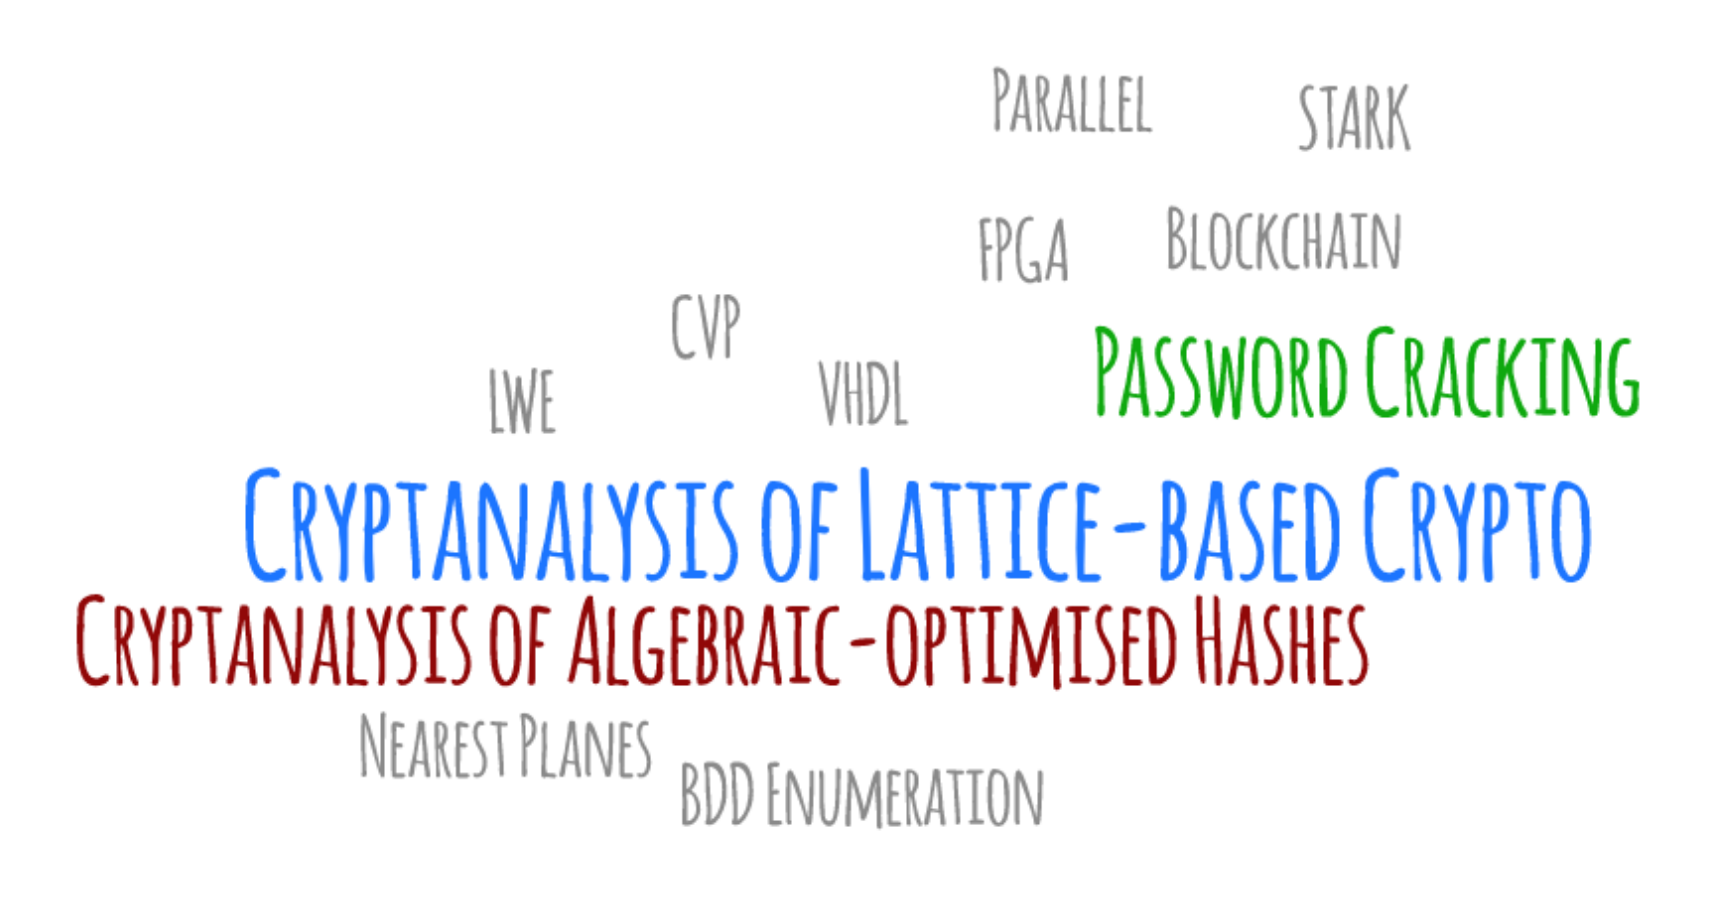
\includegraphics[width=\textwidth]{data/research-topics.png}
            \end{block}
        \end{column}
    \end{columns}
\end{frame}

\begin{frame}{High-Speed Implementation of bcrypt Password Search}
    \centering

    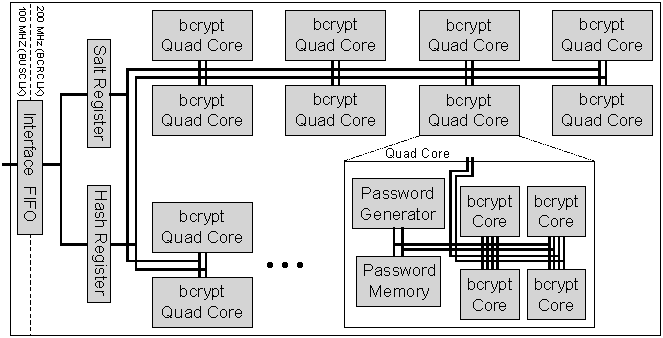
\includegraphics[height=100pt]{data/bcrypt-overview.pdf}

    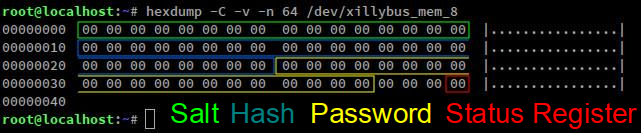
\includegraphics[width=0.75\textwidth]{data/bcrypt-mem-layout.png}
    \begin{itemize}
        \item Zedboard implementation: 4x increase to previous work
    \end{itemize}
\end{frame}

\begin{frame}{Parallel Implementation of BDD enumeration for LWE}
    \centering
    \vfill
    \only<1>{
    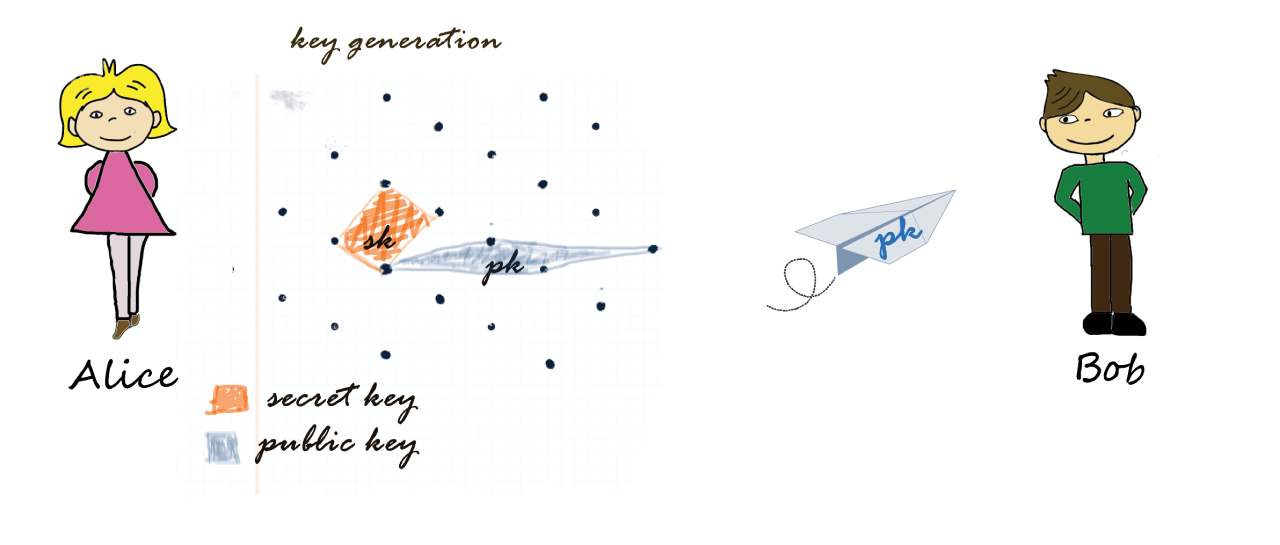
\includegraphics[height=100pt]{data/bdd-keygen-small.pdf}\\
    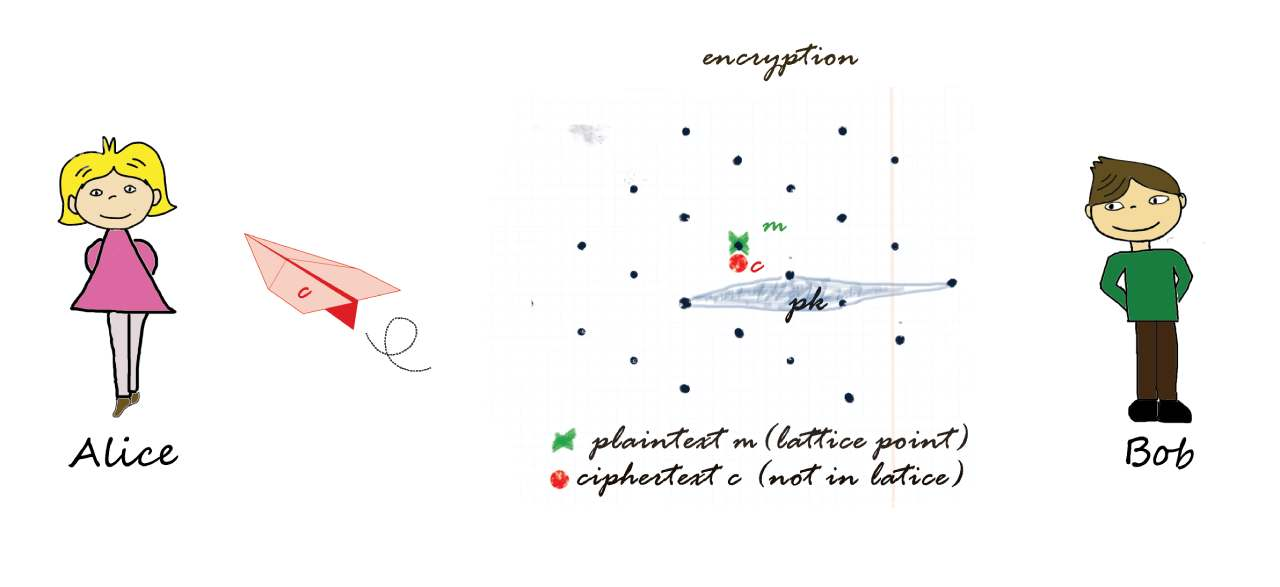
\includegraphics[height=100pt]{data/bdd-encryption-small.pdf}
    \hspace{5pt}
    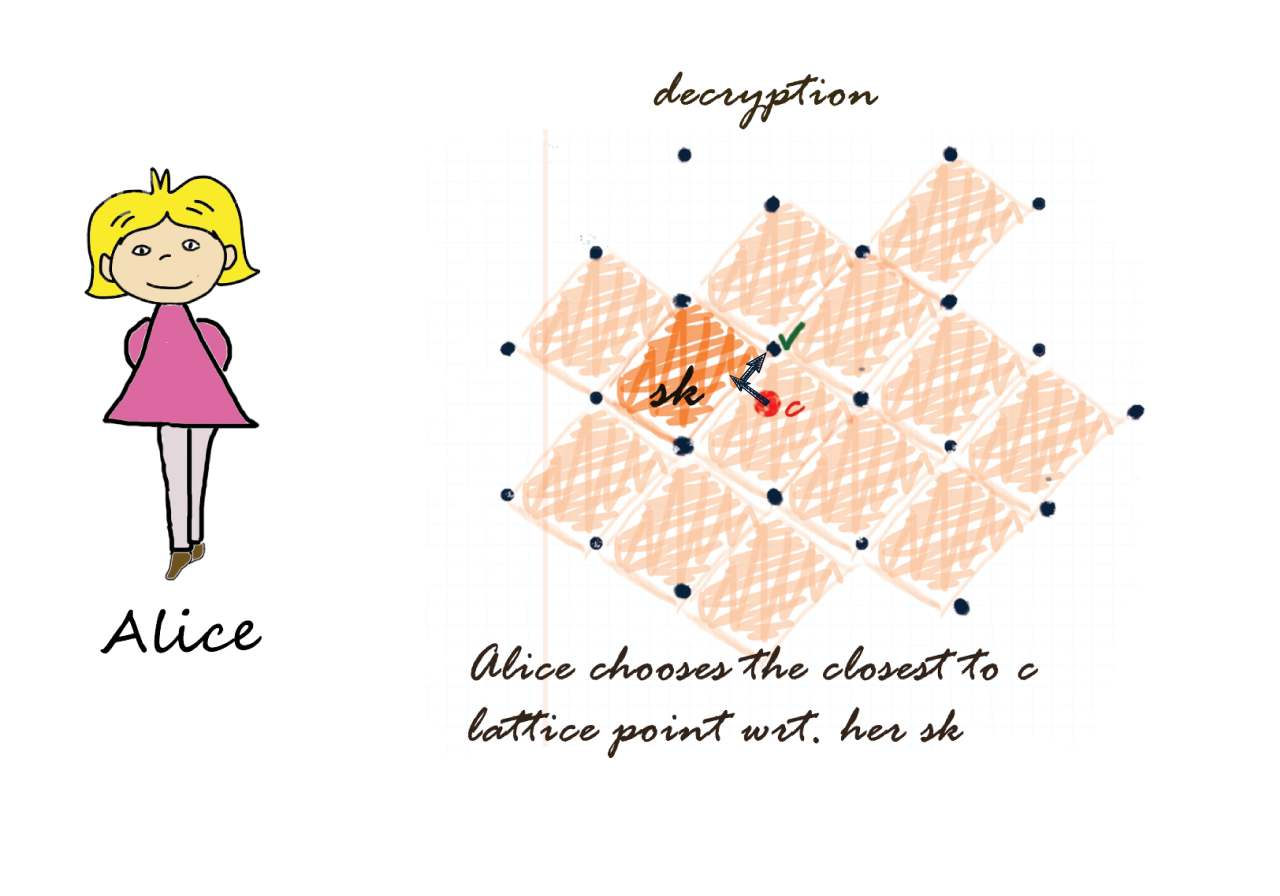
\includegraphics[height=100pt]{data/bdd-decryption-small.pdf}
    }
    \only<2>{
    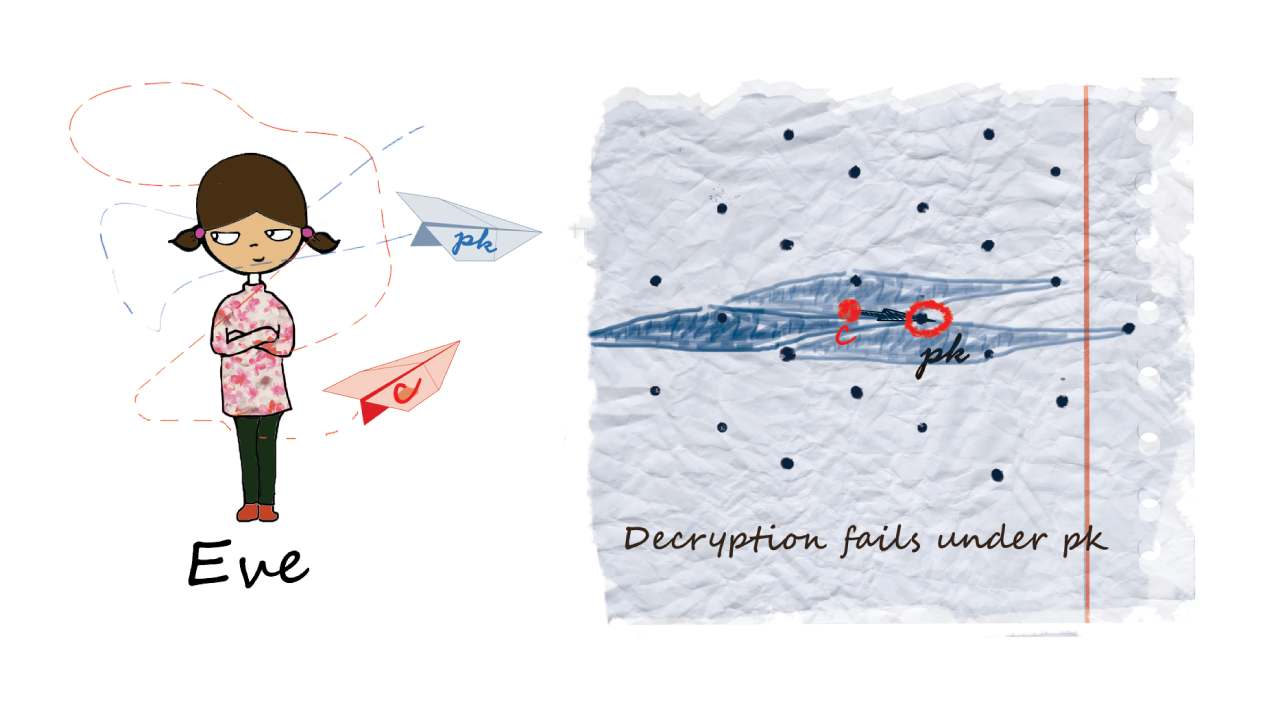
\includegraphics[height=100pt]{data/bdd-eve-small.pdf}\\
    }
    \only<3>{
    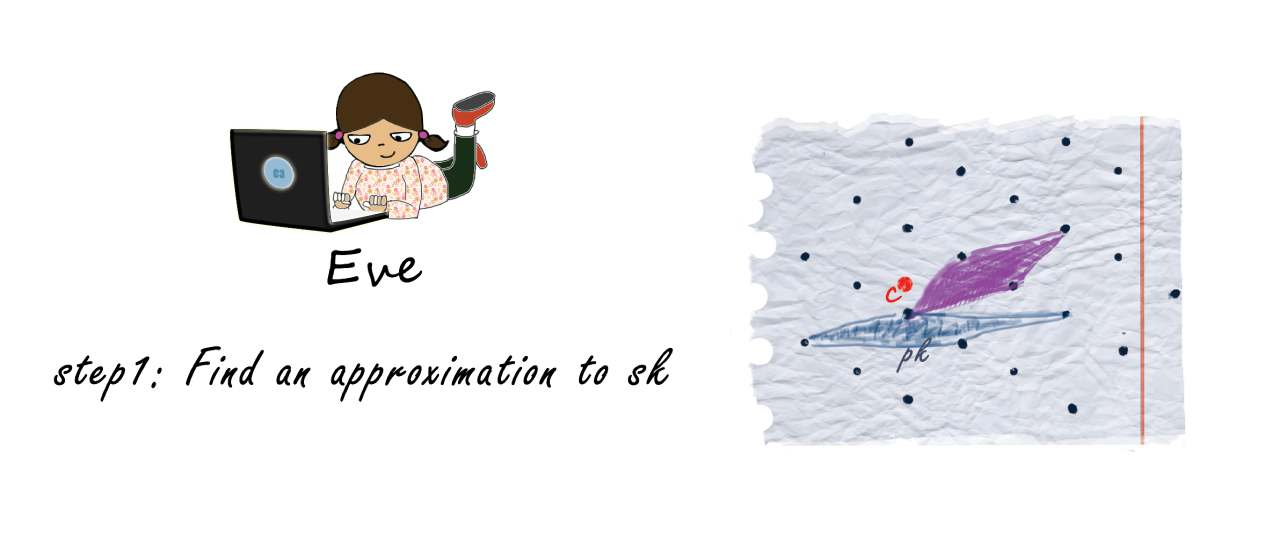
\includegraphics[height=100pt]{data/bdd-attack-step1-small.pdf}
    \hspace{5pt}
    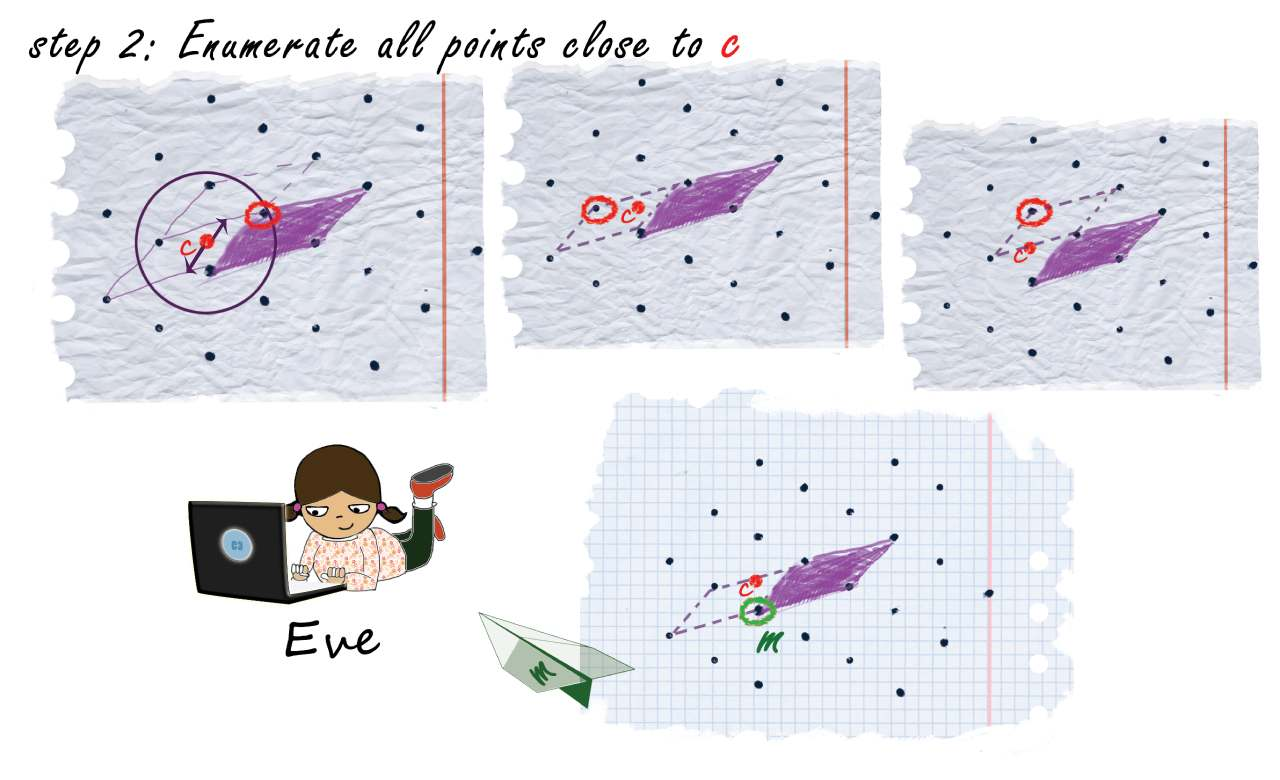
\includegraphics[height=100pt]{data/bdd-attack-step2-small.pdf}
    }
    \vfill
    \only<3>{
    \begin{itemize}
        \item Result: Enumeration step can be very good parallelized; Best Student Paper award at ACNS.
    \end{itemize}
    }
\end{frame}

\begin{frame}{Research}
    \begin{columns}
        \begin{column}{0.45\textwidth}
            \begin{itemize}
                \item \enquote{Linear Cryptanalysis: Key Schedules and Tweakable Block Ciphers}
                \item \enquote{Shorter Linear Straight-Line Programs for MDS Matrices}
                \item \enquote{Searching for Subspace Trails and Truncated Differentials}
                \item \enquote{BISON}
                \item \enquote{Observations on the DLCT and Absolute Indicators}\\[10pt]
                \item (\enquote{Spook})
            \end{itemize}
        \end{column}
        \begin{column}{0.45\textwidth}
            \setbeamercolor{block body}{use=structure,fg=black,bg=white!20!white}
            \begin{block}{Topics of PhD Thesis}
            \centering
            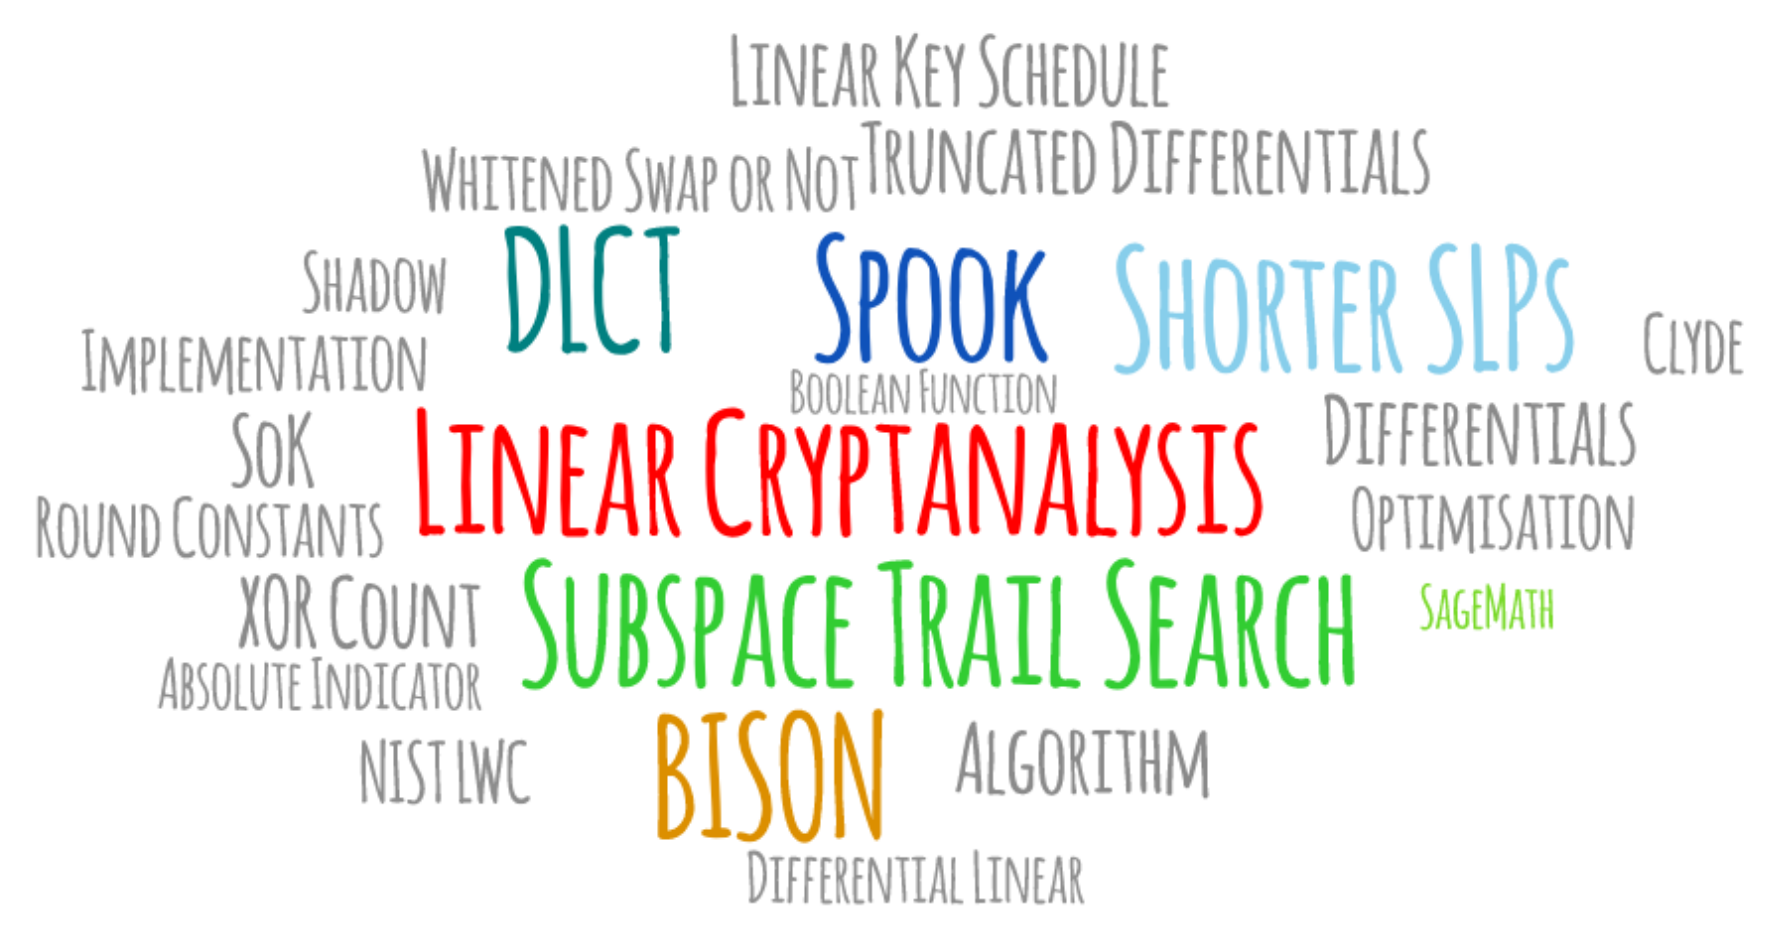
\includegraphics[width=\textwidth]{data/research-topics-thesis.png}
            \end{block}
        \end{column}
    \end{columns}
\end{frame}

\begin{frame}{Topic Classification within Symmetric Crypto}
    %\begin{center}
    \centering
        \begin{tikzpicture}
             \matrix (m) [matrix of nodes, ampersand replacement=\&, column sep=10pt, row sep=5pt] {
                 \node [draw, thick, rounded corners=10pt, color=RoyalBlue, minimum width=4cm] {\LARGE Security}; \& \node [color=alertred] {\LARGE vs.}; \& \node [draw, thick, rounded corners=10pt, color=Green, minimum width=4cm] {\LARGE Efficiency}; \& \\[10pt]
                 \node {\large SoK: Linear Cryptanalysis};                                                        \&                                      \&                                                                                  \& \node {Theory}; \\
                 \node {\large Subspace Trail Analysis};                                                          \&                                      \&                                                                                  \& \node [yshift=0.5\baselineskip, rectangle split,rectangle split parts=2] {Theory \nodepart{second} Algorithm}; \\
                                                                                                                  \&                                      \& \node {\large Shorter SLPs};                                                     \& \node {Implementation}; \\
                                                                                                                  \& \node {\large BISON};                \&                                                                                  \& \node {Instantiation}; \\
                 \node {\large DLCT};                                                                             \&                                      \&                                                                                  \& \node {Theory}; \\
                                                                                                                  \& \node {\large Spook};                \&                                                                                  \& \node {Instantiation}; \\
             };
        \end{tikzpicture}
    %\end{center}
\end{frame}

\begin{frame}{Activity in the Cryptographic Community}
    \begin{columns}
        \begin{column}{0.45\textwidth}
            \centering
            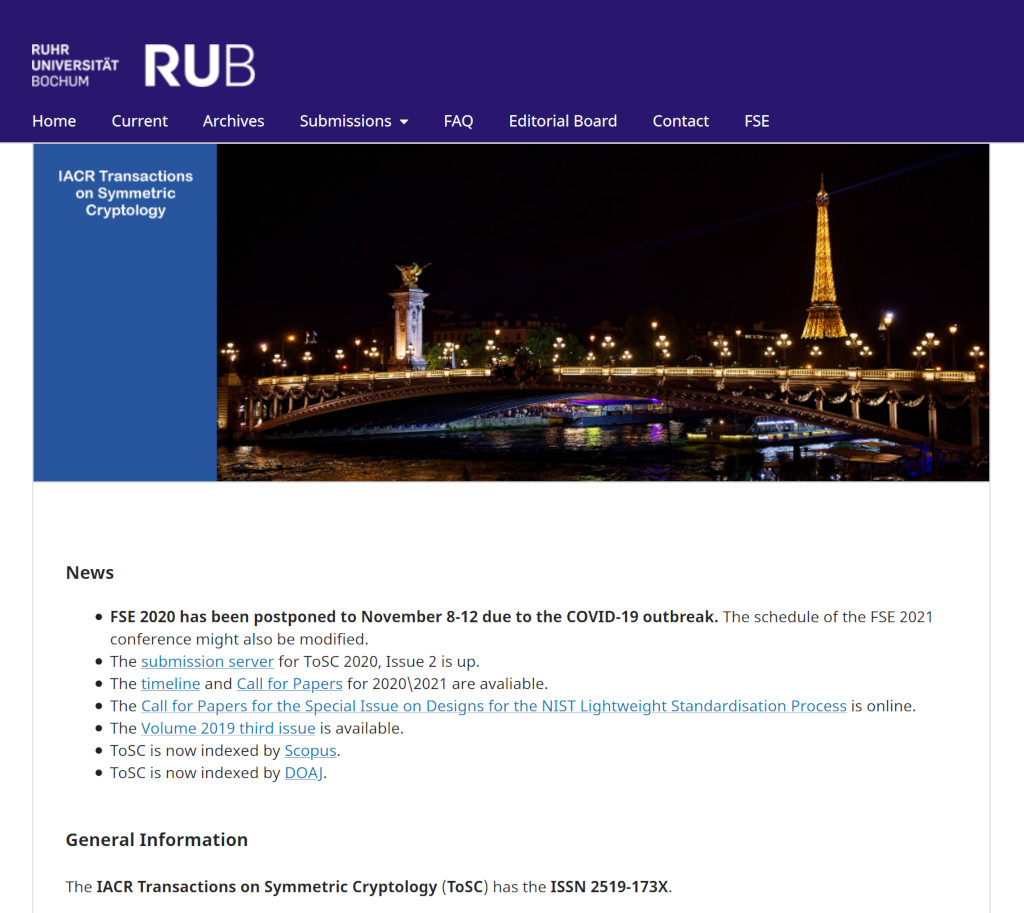
\includegraphics[width=\textwidth]{data/tosc.jpg}
        \end{column}
        \begin{column}{0.45\textwidth}
            \centering
            \vspace{-19pt}
            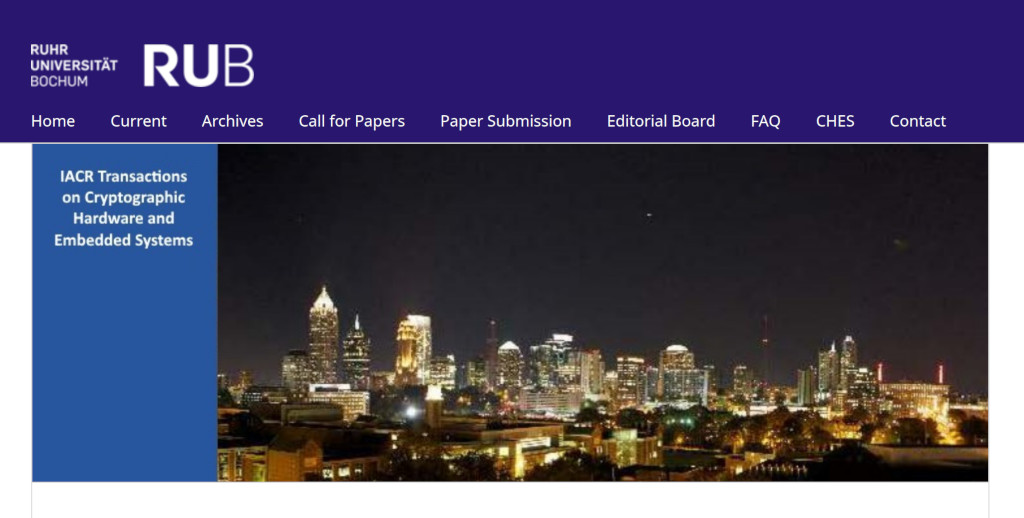
\includegraphics[width=\textwidth]{data/tches.jpg}
            \begin{itemize}
                \item IACR Conferences move to \emph{Gold Open Access} publications
                \item Published by Ruhr Uni Bochum
            \end{itemize}
        \end{column}
    \end{columns}
    \vspace{5pt}
    \visible<2>{
    \begin{itemize}
        \item NIST Lightweight Crypto Competition (LWC) round 2 candidate: Spook
    \end{itemize}
    }
\end{frame}

\begin{frame}{SageMath}
    \begin{columns}
        \begin{column}{0.5\textwidth}
            \begin{itemize}
                \item Open Source Computer Algebra System
                \item Supports Components of Cryptographic Algorithms (S-boxes, Boolean Functions)
                \item Useful to play with mathematical structures\\[10pt]
                \item Nice open source project to contribute to\\
                      (\href{https://trac.sagemath.org/query?author=~Friedrich+Wiemer&or&reviewer=~Friedrich+Wiemer&col=id&col=summary&col=status&col=owner&col=type&col=priority&col=milestone&order=priority}{my contributions})
            \end{itemize}
        \end{column}
        \begin{column}{0.45\textwidth}
            \centering
            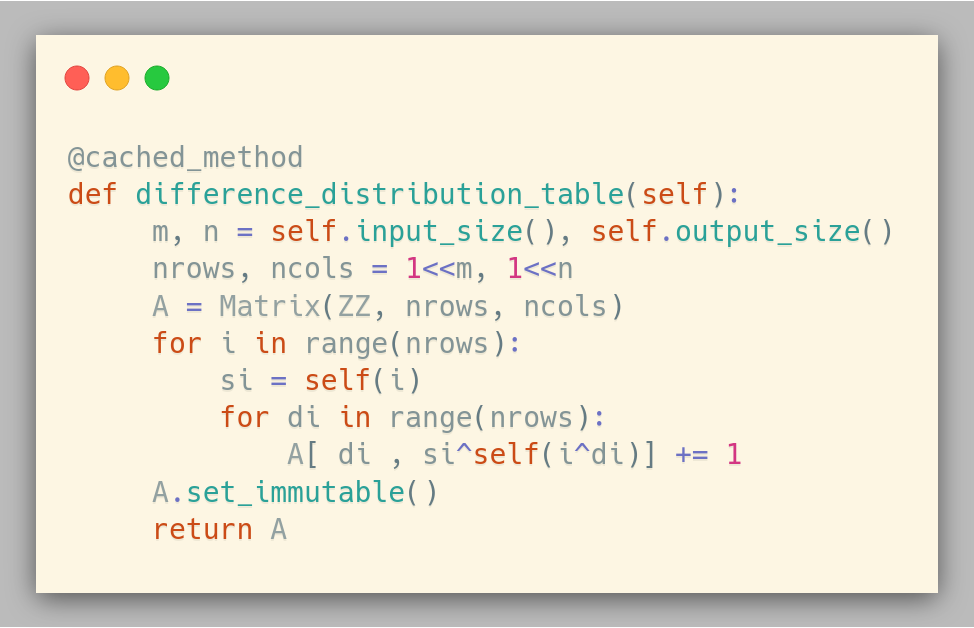
\includegraphics[height=125pt]{data/sage.png}
        \end{column}
    \end{columns}
\end{frame}

\end{document}
